\chapter{مقدّمه}
\label{fasleavval}
\label{history}
\pagenumbering{arabic}
% برای این که شماره‌گذاری صفحات از شروع فصل اول از حرفی به عددی تغییر کند باید دستور فوق را تنها بعد از فصل اول داشته باشید.
\setlatintextfont{Times New Roman}
\section{تاریخچه شبکه\nf های سلولی}

\subsubsection{نسل اوّل}
در شبکه\nf های سلولی نسل اوّل(\lr{1G})، از روش\nf های مخابرات آنالوگ استفاده می\nf شد  که مشابه رادیوهای آنالوگ عمل می\nf کردند. در مخابرات آنالوگ، از پهنای باند فرکانسی به صورت کارآمد استفاده نمی\nf شود و نسبت به سیستم\nf های دیجیتال، ظرفیت پایین\nf تری برای ارائه خدمات دارند. این سیستم\nf ها، صرفاً قادر به ارائه خدمات تماس صوتی به کاربران خود بودند. معماری \lr{1G}، در شکل \ref{1g} نشان داده\nf شده است\cite{cox}.

\begin{figure}[H]
\centering
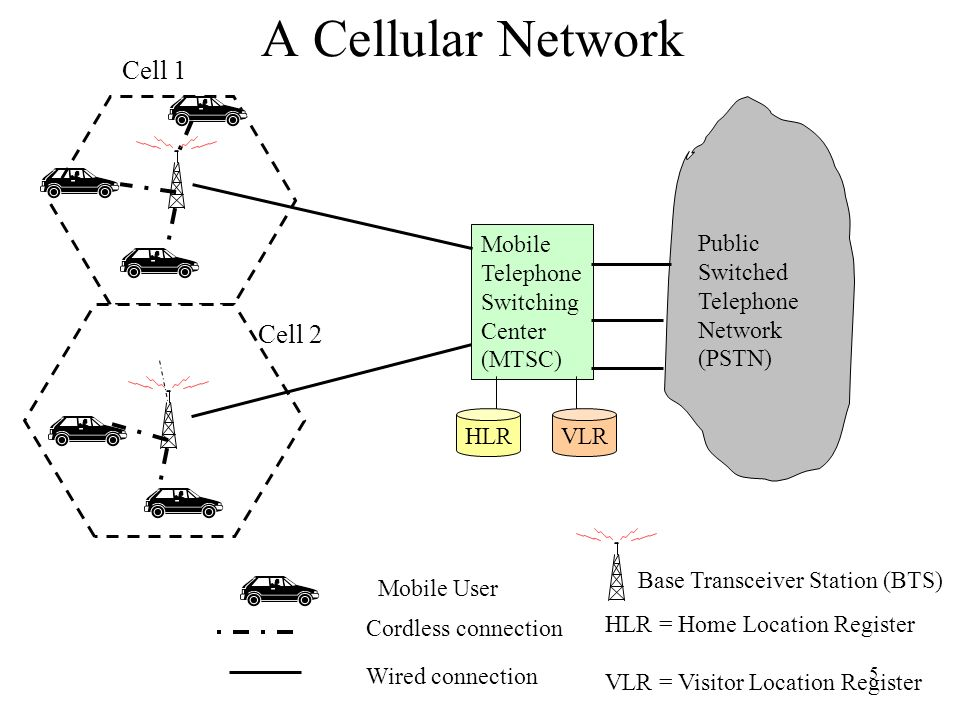
\includegraphics[width=0.7\textwidth]{1g}
\caption{معماری نسل اوّل شبکه\nf های سلولی}
\label{1g}
\end{figure}

\subsubsection{نسل دوّم}
   با ظهور نسل دوّم شبکه\nf های سلولی(\lr{2G})، برای اوّلین بار فنّاوری مخابرات دیجیتال مورد استفاده قرار گرفت. مخابرات دیجیتال، امکان استفاده بهینه\nf تر از دامنه\nf ی رادیویی را فراهم کرد. در این روش، انتقال داده\nf ها به صورت دیجیتال صورت می\nf گیرد و این امر باعث بالا رفتن کیفیت مکالمات صوتی نسب به روش آنالوگ می\nf شود. با وجود این\nf که این سیستم\nf ها در آغازِ کار، فقط برای پشتیبانی از سرویس صوتی طرّاحی شده بودند، امّا با بهبودهایی که صورت گرفت، قادر به ارائه سرویس پیامک نیز شدند. سیستم نسل دوّم \lr{GSM}\RTLfootnote{سرواژه\nf ی عبارت \lr{Global System for Mobile communication} و به معنای سیستم جهانی برای ارتباطات سیّار} که به\nf عنوان تکنولوژی مورد استفاده در اتّحادیه\nf ی اروپا طرّاحی شده بود، به محبوب\nf ترین سیستم مخابراتی در جهان تبدیل شد\cite{cox}.


   موفقیّت \lr{2G} و رشد و گسترش اینترنت، باعث شد که اپراتورهای تلفن همراه، این دو سرویس را با یکدیگر ترکیب کنند. با این کار،کاربران تلفن همراه توانستند از طریق شبکه\nf ی سلولی به اینترنت متّصل شوند. این نسل که \lr{2.5G} نامیده می\nf شود، در کنار سرویس صوتی، سرویس دیتا نیز به کاربران خود ارئه می\nf دهد. برای ارائه سرویس دیتا، باید علاوه بر شبکه\nf ی سوئیچ مداری\RTLfootnote{\lr{Circuit Switch}}، از شبکه\nf ی سوئیچ بسته\nf ای\RTLfootnote{\lr{Packet Switch}} نیز استفاده شود. همچنین، لازم است که رابط هوایی\RTLfootnote{\lr{Air Interface}: لینک ارتباطی بین دو ایستگاه در مخابرات بیسیم که شامل لایه\nf های فیزیکی و پیوند داده است.} نیز به گونه\nf ای تغییر کند که قادر به پشتیبانی از صوت و دیتا باشد. \lr{GSM} با استفاده از سرویس \lr{GPRS}\RTLfootnote{سرواژه\nf ی عبارت \lr{General Packet Radio Service}}، موارد فوق را پیاده\nf سازی کرد\cite{cox}. 
\begin{figure}[h]
\centering
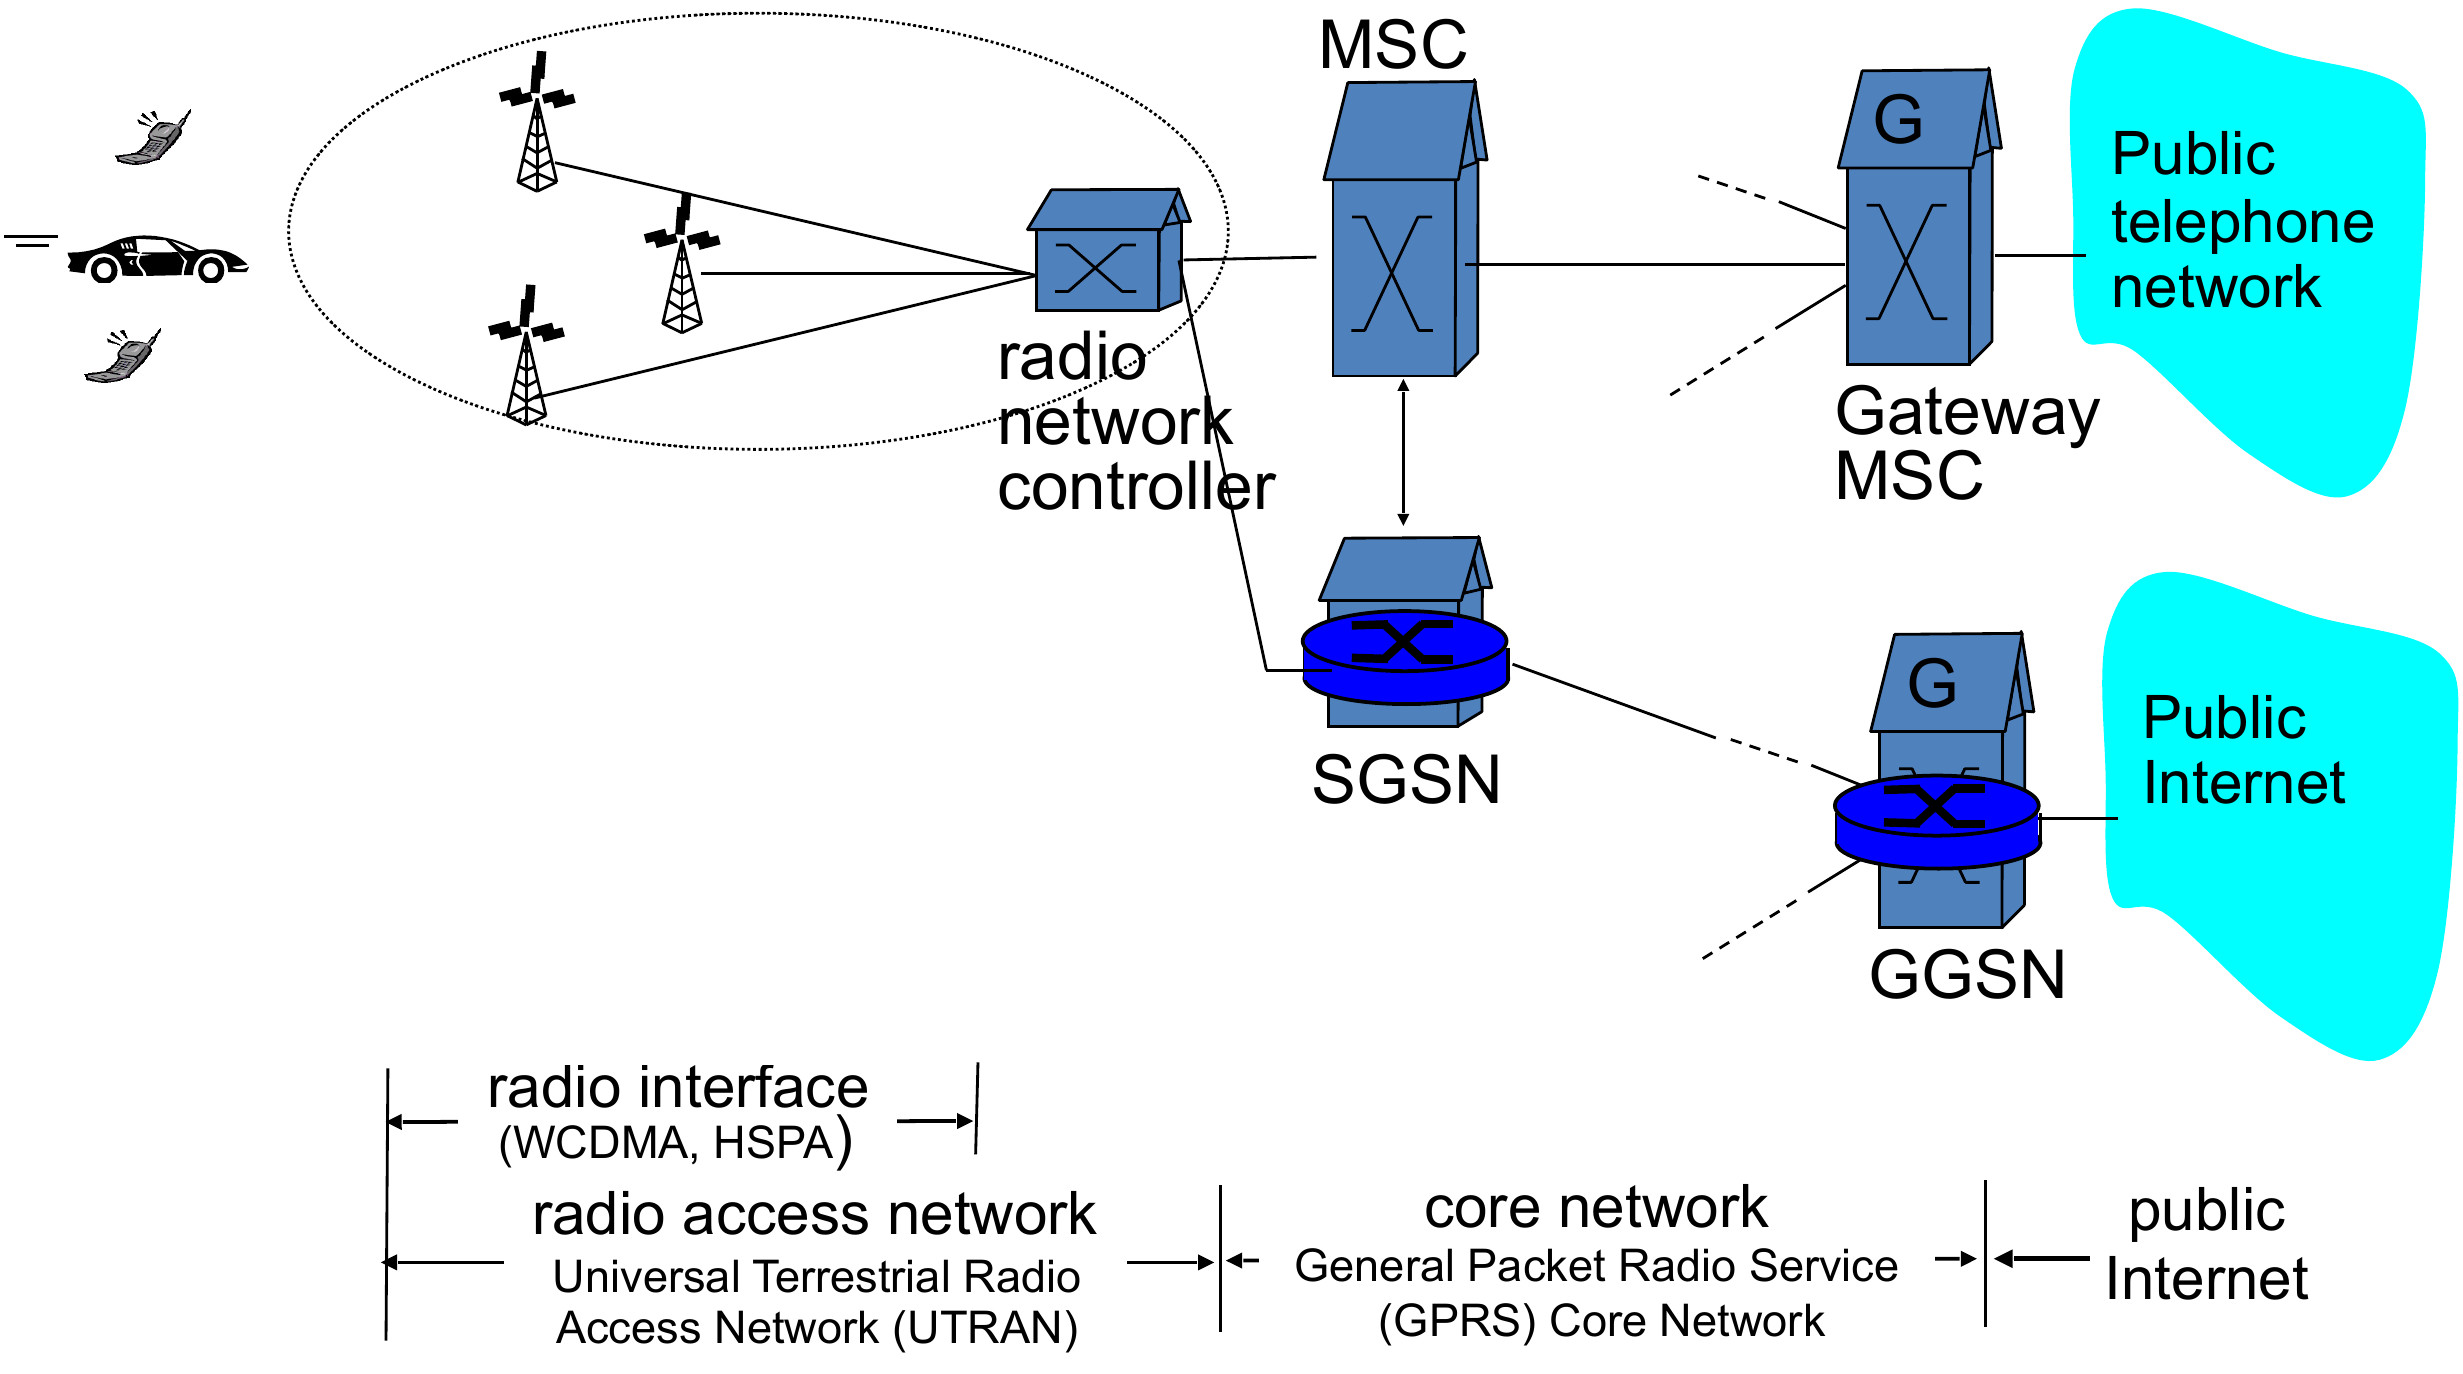
\includegraphics[width=0.7\textwidth]{3g}
\caption{معماری نسل سوّم شبکه\nf های سلولی}
\label{3g}
\end{figure}
   
\subsubsection{نسل سوّم}   
   گسترش روز افزون اینترنت و نیاز کاربران به اینترنت سریع\nf تر و حجم دیتای بیشتر، تحوّلی دیگر در حوزه\nf ی شبکه\nf های سلولی رقم زد. در ابتدا، طرّاحان با استفاده از روش\nf هایی مانند \lr{EDGE}\RTLfootnote{سرواژه\nf ی عبارت \lr{Enhances Data rate for GSM Evolution}}، کارایی سیستم\nf های \lr{2G} و \lr{2.5G} را افزایش دادند. پس از آن، نسل سوّم شبکه\nf های سلولی(\lr{3G}) معرّفی شد. در نسل سوّم، هسته\nf ی شبکه\nf ی سلولی تغییری نکرد امّا تکنولوژی ناحیه\nf ی دسترسی رادیویی، به\nf طور کامل تغییر کرد. در ناحیه\nf ی دسترسی رادیویی نسل سوّم، از تکنولوژی \lr{WCDAM}\RTLfootnote{سرواژه\nf ی عبارت \lr{Wideband Code Division Multiple Access}} و یا \lr{TD-SCDMA}\RTLfootnote{سرواژه\nf ی عبارت \lr{Time Division Synchronous Code Division Multiple Access}} استفاده می\nf شود. این روش\nf ها، باعث شد که \lr{3G} بتواند از حداکثر نرخ ارسال داده\nf ی\RTLfootnote{\lr{Maximum Data Rate}} بیشتری پشتیبانی کند. در \lr{3G} نیز مانند \lr{2.5G}، شبکه\nf ی دیتا کار خود را به صورت موازی با شبکه سرویس صوتی انجام می\nf دهد. معماری \lr{3G}، در شکل \ref{3g} نشان داده\nf شده است\cite{cox}.



\subsubsection{نسل چهارم}
 تفاوت اصلی نسل چهارم(\lr{4G}) با نسل\nf های قبل از خود، عدم پشتیبانی از شبکه\nf ی سوئیچ مداری است. در این نسل، تماس صوتی نیز از طریق شبکه سوئیچ بسته\nf ای برقرار می\nf شود. از آنجایی\nf که شبکه\nf های سوئیچ بسته\nf ای، به\nf  طور ذاتی و اوّلیه، کیفیّت سرویس(\lr{QoS}) را تضمین نمی\nf کنند، نیاز به تمهیدات خاص و جداگانه\nf ای برای فراهم کردن کیفیت سرویس و ارائه\nf ی سرویس صوتیِ باکیفیت می\nf باشد. همچنین در این نسل، استفاده از فنّاوری\nf هایی مانند \lr{MIMO}\RTLfootnote{سرواژه\nf ی عبارت \lr{Multiple Input and Multiple Output} و به معنای چند ورودی و چند خروجی} و سلول\nf های کوچک، باعث افزایش کارایی و نرخ دیتا شده است. معماری \lr{4G}، در شکل \ref{4g} نشان داده\nf شده است\cite{cox}.
 \begin{figure}[H]
 \centering
 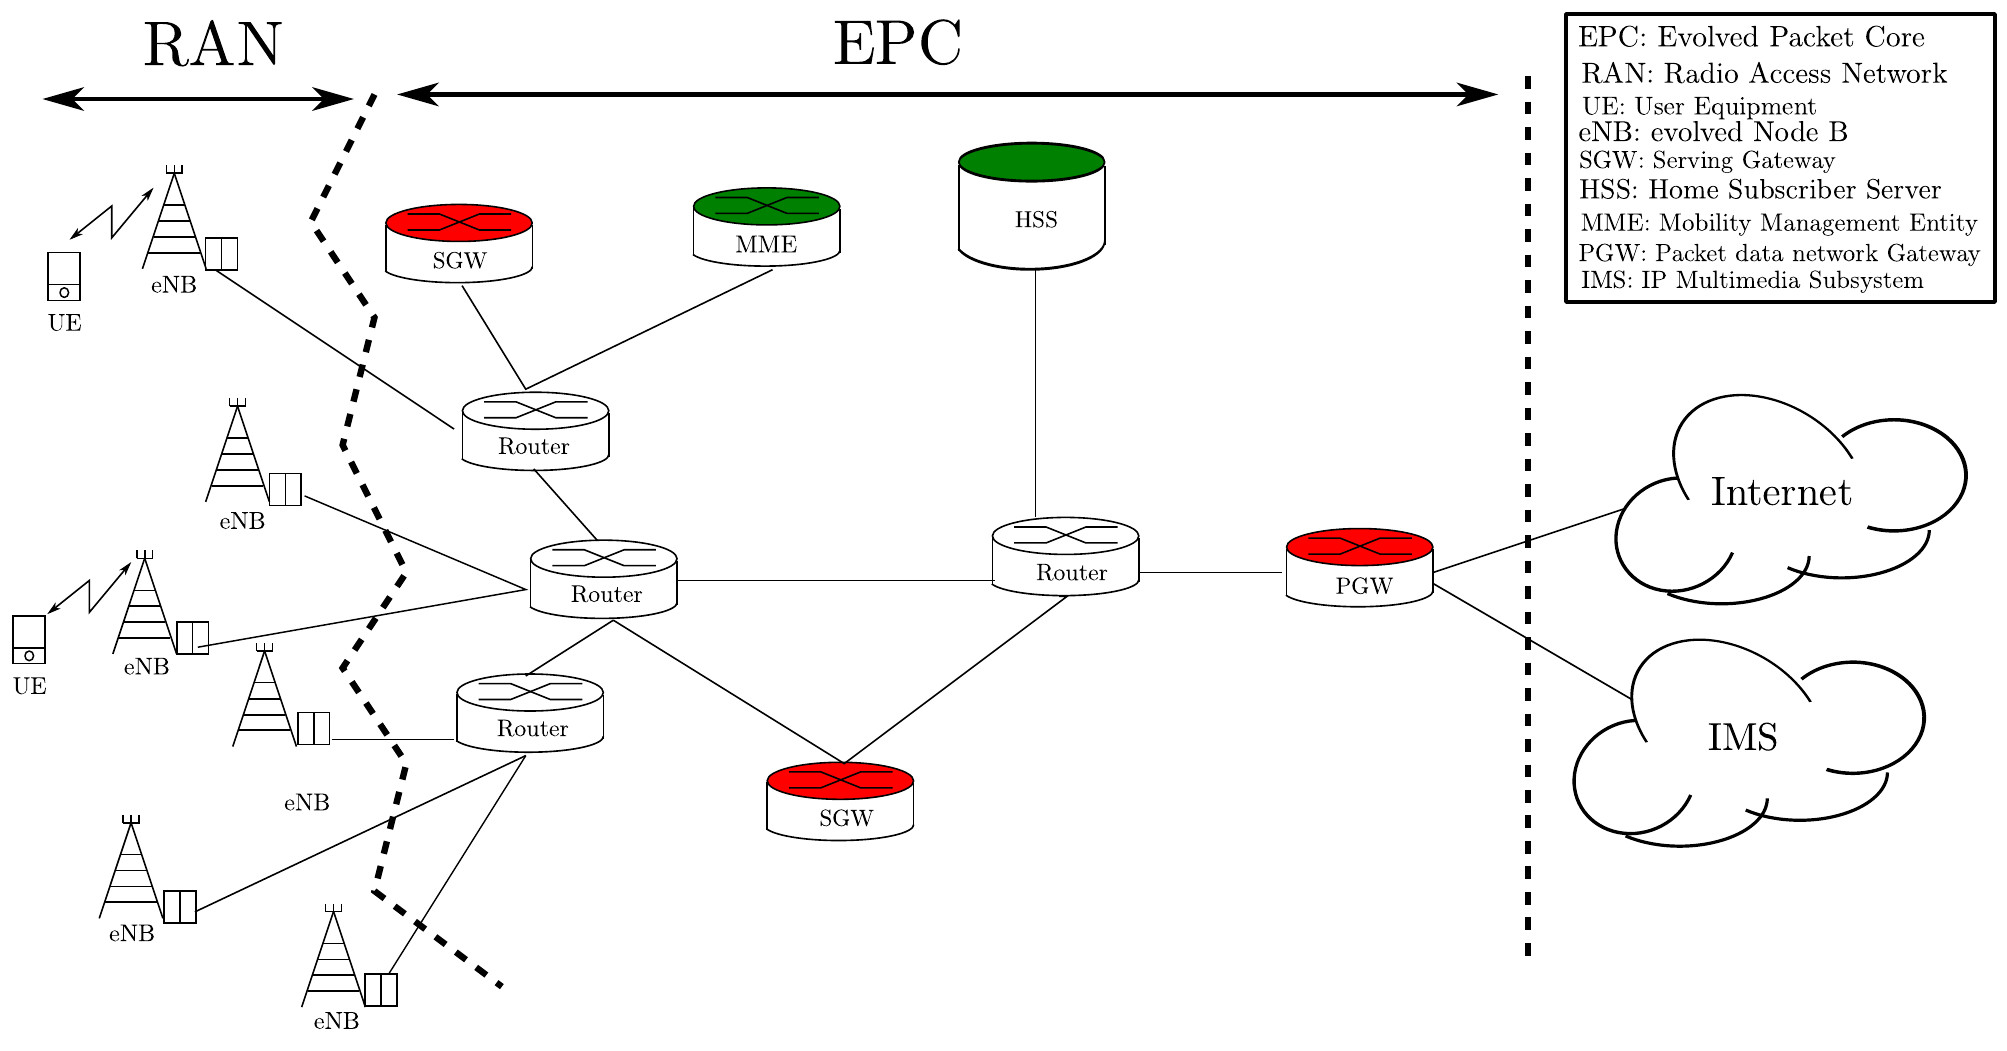
\includegraphics[width=\textwidth]{4g}
 \caption{معماری نسل چهارم شبکه\nf های سلولی}
 \label{4g}
 \end{figure}

%\begin{figure}[h]
%\centering
%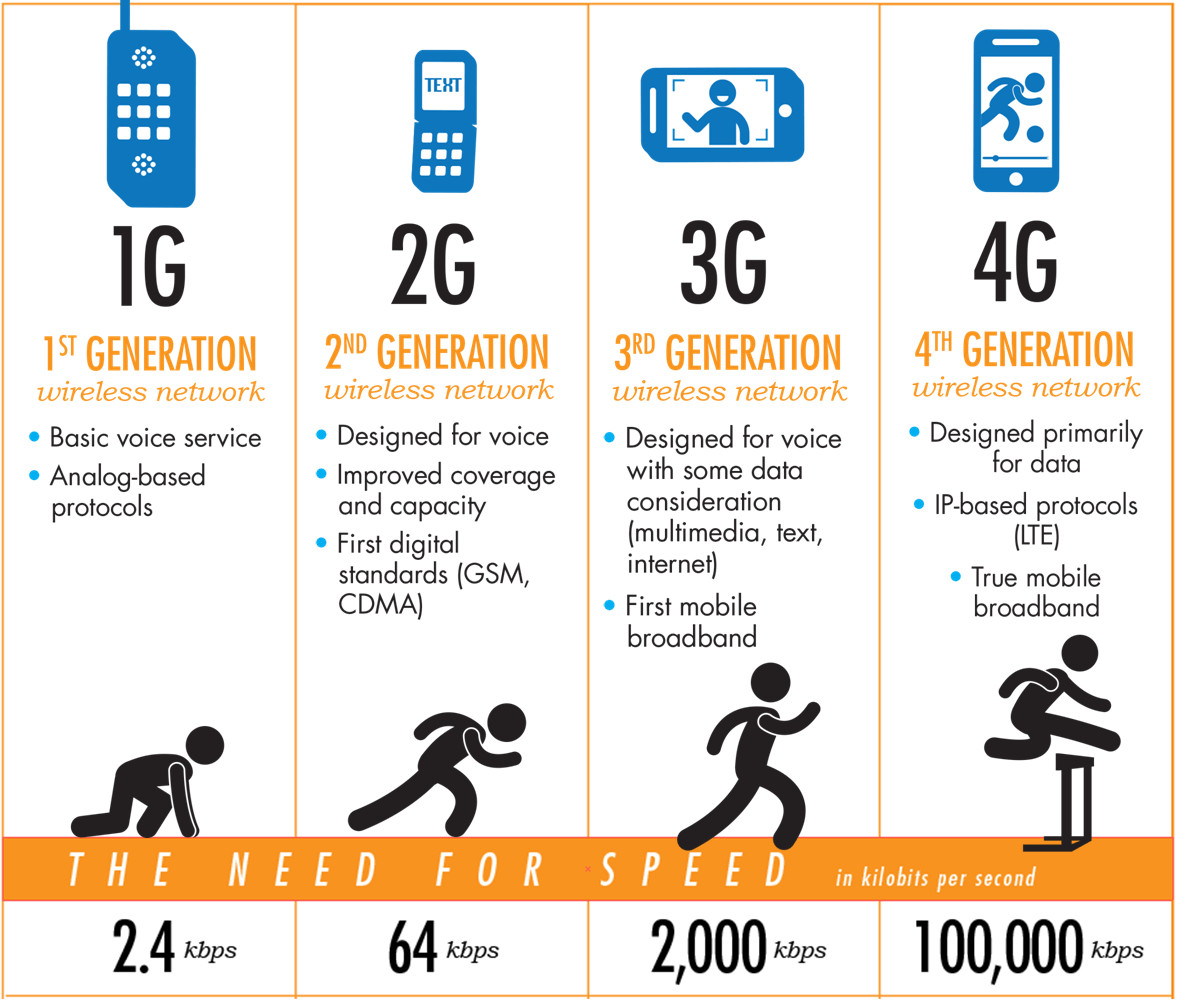
\includegraphics[width=0.75\textwidth]{evolution}
%\caption{سیر تکامل شبکه\nf های سلولی از نسل ۱ تا ۴}
%\label{evolve}
%\end{figure}
 
\subsubsection{نسل پنجم}
نیازمندی\nf ها و استانداردهای کمّی و کیفی تعریف\nf شده برای نسل پنجم شبکه\nf های سلّولی(\lr{5G})، باعث تفاوت قابل توجّه این نسل، با نسل\nf های پیشین خود می\nf شود. ظرفیّت\RTLfootnote{\lr{Throughput}} بالا، تأخیر کم، پشتیبانی از تعداد زیادی کاربر و مصرف توان کم، از جمله این موارد می\nf باشد. حدّاکثر نرخ دیتا در \lr{5G}، بیش از ۱۰۰۰ برابر بیشتر از \lr{4G} است و این موضوع، خود بیانگر تحوّلی بزرگ در شبکه\nf های سلولی است.]
\begin{figure}[h]
\centering
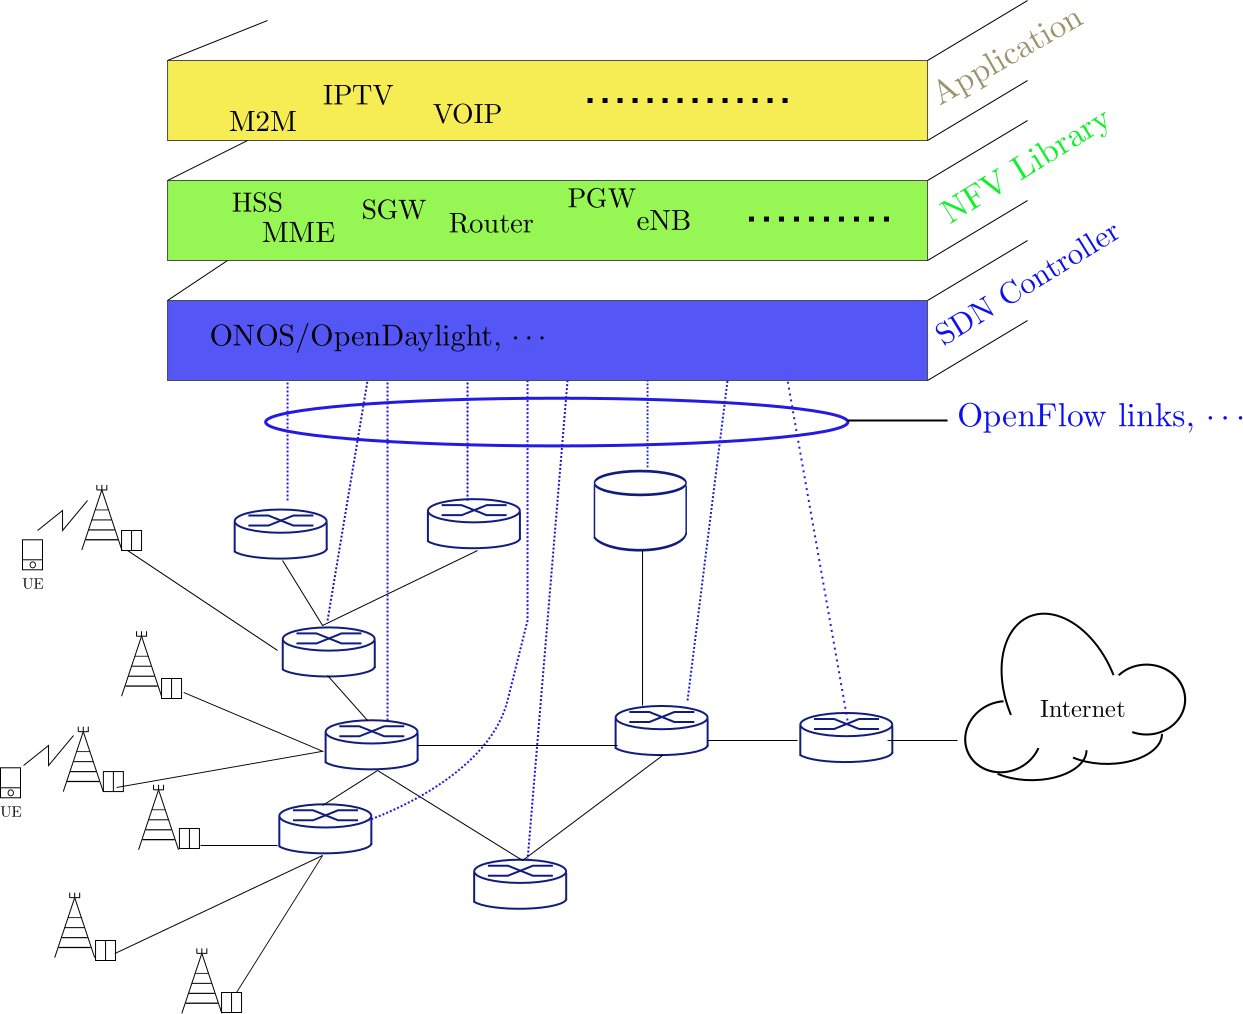
\includegraphics[width=0.75\textwidth]{5g}
\caption{معماری نسل پنجم شبکه\nf های سلولی}
\label{5g}
\end{figure}
از آنجایی\nf که برای دستیابی به این استانداردها و نیازمندی\nf ها،  منابع بسیار زیادی مورد نیاز است، \lr{5G} راه\nf حل\nf های جایگزینی برای این کار ارائه می\nf دهد. بیشتر این راه\nf حل\nf ها، بر اساس روش\nf های \lr{softwarization}\RTLfootnote{پیاده\nf سازی نرم\nf افزاری شبکه (\lr{software defined network})}، \lr{virtualization}\RTLfootnote{مجازی\nf سازی}و \lr{cloudificatoin}\RTLfootnote{انتقال دادن سرویس بر روی ابر} می\nf باشند.


\section{دلایل پیدایش \lr{IMS}}
همانطور که در بخش \ref{history} توضیح داده\nf شد، طبق استادنداردهای نسل ۴ به بعد، تماس\nf های صوتی باید از طریق سوئیچ\nf های بسته\nf ای منتقل شوند. بسیاری از اپراتورهای تلفن همراه، ادّعا می\nf کنند که نسل چهارم ارتباطات را پیاده\nf سازی کرده\nf اند، امّا این امر بیشتر در زمینه\nf ی پهنای باند و افزایش سرعت اینترنتِ همراه محقّق شده است. هنوز بسیاری از اپراتورهای تلفن همراه، تماس\nf های صوتی را از طریق سوئیچ\nf های مداری برقرار می\nf کنند. هنگامی که شما اینترنت نسل ۴ را در اختیار دارید و در نوار وضعیت تلفن همراه شما علامت \lr{4G} نمایش داده می\nf شود، اگر اقدام به برقراری تماس تلفنی کنید یا کسی با شما تماس بگیرد، متوجّه خواهیدشد که علامت \lr{4G} در نوار وضعیت، به علامت \lr{H}\RTLfootnote{حرف \lr{H}، به عنوان نماد عبارت \lr{HSPA} به کار می\nf رود. عبارت \lr{HSPA}، سرواژه\nf ی \lr{High Speed Access Packet} و به معنی دسترسی سریع به بسته\nf ها است. این عبارت، نام تکنولوژی اینترنت نسل سوّم ارتباطات است. } تغییر میابد. دلیل این تغییر وضعیت، عدم پشتیبانی اپراتور موردنظر(به\nf خصوص اپراتورهای ایرانی همراه اوّل، ایرانسل و رایتل) از برقراری تماس تلفنی مبتنی بر تکلنولوژی نسل ۴ است؛ لذا این اپراتورها، سرویس اینترنت را با استفاده از تکلنولوژی نسل چهارم و سرویس تماس صوتی را با استفاده از تکنولوژی نسل سوّم ارائه می\nf دهند.

راه\nf حلی که برای مشکل مذکور به ذهن می\nf رسد، استفاده از تکنولوژی \lr{VOIP}\RTLfootnote{سرواژه\nf ی عبارت \lr{Voice Over IP} و به معنای صدا بر روی \lr{IP}} به جای سوئیچ\nf های مداری است. از آنجایی که اپراتورهای تلفن همراه، شبکه\nf ی داخلی مخصوص به خود را دارند و کاربر با اتّصال به ایستگاه\nf های مخابراتی\RTLfootnote{\lr{Base Station}}، می\nf تواند آدرس \lr{IP} به دست آورد، بدیهی است که می\nf تواند از سرویس \lr{VOIP} استفاده کند و با استفاده از این سرویس، تماس صوتی برقرار نماید. اپراتور موردنظر نیز می\nf تواند با استفاده از درگاه\nf های مختلف، برقراری تماس بین مشترک خود و مشترکین خارج از شبکه\nf ی خود(چه مشترکین سایر اپراتورها و چه مشترکین تلفن ثابت) را فراهم کند.

مشکل اصلی راه\nf حل فوق، عدم تضمین کیفیّت سرویس است؛ به این معنی که با وجود بالا بودن کیفیّت ارتباط دستگاه کاربر با ایستگاه مخابراتی\RTLfootnote{بالا بودن نسبت سیگنال به نویز که به آن \lr{Signal to Noise Ratio} یا با اختصار \lr{SNR} می\nf گویند. زمانی که\lr{SNR} بالا باشد، کاربر قادر است اطّلاعات زیادی را در زمان کم و به درستی، به ایستگاه مخابراتی بفرستد.} ، ممکن است کاربر نتواند تماس صوتی برقرار کند یا تماس صوتی با کیفیّت پایین را تجربه کند. دلیل اصلی این مشکل، وجود تراکم\RTLfootnote{Congestion} در لینک\nf های داخلی و یا نودهای\RTLfootnote{مسیریاب\nf ها و سوئیچ\nf های درون شبکه} شبکه\nf ی اپراتور می\nf باشد. همچنین، ممکن است تعداد زیادی کاربر به یک ایستگاه مخابراتی متّصل شده باشند. از آنجایی که ایستگاه مخابراتی، باند فرکانسی\RTLfootnote{البتّه روش\nf های دیگر تقسیم مانند تقسیم زمان و ... نیز مورد استفاده قرار می\nf گیرند.} خود را بین تمام این کاربران تقسیم می\nf کند، به کاربران سهم کم\nf تری از باند فرکانسی می\nf رسد و در نتیجه، نرخ ارسال و دریافت دیتای کاربران پایین می\nf آید. بنابراین مشکل عدم امکان برقراری تماس و یا تماس با کیفیّت پایین به\nf وجود می\nf آید. از آنجایی\nf که اپراتورهای تلفن همراه، موظّف به ارائه\nf ی سرویس تماس صوتیِ باکیفیت در بیشتر نقاط جغرافیایی هستند و همچنین وجود اهمیّت برقراری تماس صوتی در شرایط مختلف و خاص، در صورت تحقّق نشدن این امر، مشکلات زیادی به\nf وجود خواهدآمد. جریمه شدن اپراتور موردنظر به دلیل عدم توانایی ارائه\nf ی سرویس مناسب و همچنین نارضایتی مشترکین آن اپراتور، اصلی\nf ترین مشکلات پیشِ رو هستند.

از آنجایی\nf که اهمیّت امکان برقراری تماس صوتی و همچنین کیفیّت سرویس در تماس صوتی(یا ویدیوئی) بسیار حیاتی\nf تر از سایر سرویس\nf ها مانند سرویس دریافت فایل از اینترنت است، می\nf توان تدابیری اندیشید تا بسته\nf های مربوط به تماس صوتی، اولويّت بیشتری برای مسیریابی و گذر از شبکه داشته باشند. با انجام این کار، مشکل مذکور حل خواهد شد. با پیکربندی سرورهای \lr{VOIP} و همچنین نودهای داخلی شبکه\nf ی اپراتور، می\nf توان این عمل را انجام داد؛ امّا باز هم یک مشکل اساسی باقی خواهدماند. سرویس\nf های متداول \lr{VOIP}، قادر نیستند که با تعامل با المان\nf های معماری نسل چهارم و پنجم، پهنای باند تضمین\nf شده\nf ای را برای کاربر فراهم کنند؛ به این معنی که نمی\nf توانند به\nf وسیله\nf ی ارتباط با یک ایستگاه مخابراتی که دستگاه کاربر به آن متّصل است، از ایستگاه مخابراتی بخواهند که به کاربر مورد نظر، سهم بیشتری از باند فرکانسی و شبکه\nf ی دسترسی رادیویی\RTLfootnote{\lr{Radio Access Network} که به آن \lr{RAN} می\nf گویند.} اختصاص دهد تا کاربر بتواند تماس صوتیِ باکیفیّت برقرار کند. همچنین، در صورت استفاده از سرویس \lr{VOIP}، ایجاد تماس صوتی بین مشترکین یک اپراتور با مشترکین تلفن ثابت و مشترکین سایر اپراتورها، دشواری\nf های خاصی را به وجود می\nf آورد.

وجود مسائل و مشکلات فوق، باعث شکل\nf گیری سیستم جدیدی به نام \lr{IMS}\RTLfootnote{سرواژه\nf ی عبارت \lr{IP Multimedia Subsystem}} شد. استانداردهای این سیستم، توسّط سازمان \lr{3gpp} تدوین شده\nf اند. سیستم \lr{IMS} را می\nf توان تکامل سیستم\nf های \lr{VOIP} دانست. سیستم \lr{IMS}، به\nf راحتی می\nf تواند با المان\nf های معماری نسل چهارم و پنجم ارتباطات تعامل کند و برخورداری از کیفیّت سرویس در تماس\nf های صوتی(یا ویدیوئی) را برای کاربران فراهم کند. المان\nf های پیاده\nf سازی\nf شده در \lr{IMS}، ایجاد تماس صوتی بین مشترکین یک اپراتور با مشترکین سایر اپراتورها، مشترکین تلفن ثابت و همچنین مشترکین سرویس\nf های \lr{VOIP} را بسیار آسان می\nf کند. 

استفاده از \lr{IMS}، راهی برای کنار گذاشتن سوئیچ\nf های مداری و ورود به عرصه\nf ی سوئیچ\nf های بسته\nf ای در صنعت مخابرات است. با استفاده از \lr{IMS}، هزینه\nf های شبکه و سایر هزینه\nf های اپراتورها کاهش میابد و اپراتورها، قادر به ارائه\nf ی سرویس\nf های جدید و نوظهور، در کنار سرویس\nf های قبلی خود می\nf شوند. مشترکین اپراتورها، از سرویس\nf های جدیدی بهره\nf مند می\nf شوند و سرویس\nf های قبلی را با کیفیّت بیشتری تجربه می\nf کنند\cite{blended}.

همان\nf طور که در شکل \ref{4g} دیده می\nf شود، المان \lr{PGW}، نقطه\nf ی اتّصال \lr{IMS} به شبکه\nf ی نسل چهارم ارتباطات است.  در واقع، نقطه\nf ی اتّصال \lr{IMS} به شبکه\nf های سلولی، همان نقطه\nf ای است که شبکه\nf ی سلولی را به شبکه\nf ی اینترنت وصل می\nf کند. لذا، برای اتّصال \lr{IMS} به شبکه\nf ی \lr{5G} نیز از المان \lr{PGW} استفاده می\nf شود.

\section{کارهای انجام\nf شده}

در این پروژه، ابتدا تحقیقات و مطالعاتی در مورد \lr{IMS} و معماری آن و همچنین، مزایا و کاربردهای این سیستم انجام شد. پس از بررسی پیاده\nf سازی\nf های مختلف \lr{IMS}، پیاده\nf سازی متن\nf باز \lr{clearwater}(بخش \ref{cwpart}) انتخاب شد. \lr{clearwater} را می\nf توان به\nf صورت توزیع\nf شده و یا یکپارچه پیاده\nf سازی کرد. پیاده\nf سازی\nf های توزیع\nf شده، برای پشتیبانی از تعداد زیادی کاربر مورد استفاده قرار می\nf گیرند؛ در حالی که پیاده\nf سازی\nf های یکپارچه برای امور تحقیقاتی و همچنین آشنایی با این سیستم مورد استفاده قرار می\nf گیرند. لذا، پیاده\nf سازی یکپارچه بر روی سکّوی مجازی\nf سازی انجام شد و از طریق آن، تماس تلفنی در بستر شبکه\nf ی داخلی دانشگاه\RTLfootnote{از هر شبکه\nf ای که مبتنی بر پروتکل اینترنت است می\nf توان استفاده کرد.} صورت گرفت. این تماس تلفنی، بین کاربران تلفن همراه و همچنین کاربران رایانه\nf ی شخصی صورت گرفت و کیفیت مطلوبی داشت (بخش \ref{cwaio}). پس از برقراری تماس تلفنی، کارکردهای سیستم مورد آزمایش قرار گرفت. این آزمایش، به\nf وسیله\nf ی کدهای آماده\nf ای که \lr{clearwater} در اختیار قرار داده است، انجام شد(بخش \ref{livetestPart}). 

سپس، تحقیقاتی در مورد تأمین کیفیت سرویس توسّط این سیستم انجام شد. مقایسه\nf ی کیفیت سرویس در \lr{IMS} و سیستم\nf های \lr{VOIP} متداول، در دو بخش صورت گرفت. در بخش اوّل که از \lr{IMS} به\nf عنوان یک ارائه\nf دهنده\nf ی سرویس \lr{VOIP} در بستر شبکه\nf ی محلّی استفاده می\nf شود، کیفیت سرویس در مدیای\RTLfootnote{\lr{Media}} مبادله\nf شده مقایسه شد. سپس، سیگنالینگ\nf های \lr{IMS} با سیگنالینگ\nf های یکی از سرویس\nf های \lr{VOIP} متداول مقایسه شدند. برای انجام این کار، سیستم \lr{VOIP} متن\nf باز \lr{Asterisk} پیاده\nf سازی شد و بسته\nf های مبادله\nf شده مورد ارزیابی و بررسی قرار گرفتند. در بخش دوّم نیز، کیفیت سرویس \lr{IMS} در صورت استفاده در شبکه\nf های سلولی، با کیفیت سیستم\nf های \lr{VOIP} مورد مقایسه قرار گرفتند. 

مستندات و تالار گفتمان \lr{clearwater} نیز برای آشنایی بیشتر با این سیستم و یادگیری استفاده از قابلیت\nf های آن، مورد مطالعه قرار گرفت. سپس، شبکه\nf ی سلولی نسل چهارم(\lr{4G}) با استفاده از پروژه\nf ی کارشناسی یکی از دانشجویان دانشکده برق و کامپیوتر و به\nf صورت نرم\nf افزاری پیاده\nf سازی شد. کاربران این شبکه، می\nf توانستند از طریق سیم\nf کارت، به این شبکه متّصل شوند و از طریق آن، به اینترنت دسترسی داشته\nf باشند. با اتّصال \lr{IMS} به این شبکه به\nf عنوان سرور \lr{VOIP}، کاربران تلفن همراه، از طریق سیم\nf کارت و بدون استفاده از ارتباط وای\nf فای، تماس تلفنی برقرار کردند.

پس از آشنایی کامل با پیکربندی و کارکرد المان\nf های مختلف معماری \lr{clearwater}، نحوه\nf ی ارتباط این سیستم با شبکه\nf ی تلفن ثابت مورد بررسی قرار گرفت. به دلیل عدم دسترسی به\nf موقع به تجهیزات سخت\nf افزاری و نرم\nf افزاری موردنیاز برای ایجاد این ارتباط، پیاده\nf سازی عملی صورت نگرفت و انجام این کار، به زمان آینده موکول شد. توضیحات لازم در مورد نحوه\nf ی ارتباط این دو سیستم به یکدیگر، در پیوست (\ref{pstnPart}) آورده شده است.